\documentclass[english,a4paper,twocolumn,article,10pt]{memoir}		
\usepackage[utf8x]{inputenc}	
\usepackage{graphicx}		

\usepackage{mathtools}
\usepackage{hyperref}	


% Format of infinitesimal fx. as integration-variable
\newcommand\dx[1]{\,\text{d}#1}


\title{Besselfunctions of the first kind} 

\author{Johannes Kruse}
\date{\today}


\begin{document}

\maketitle
The following text is pulled from wikipedia: \url{http://www.sharelatex.com}

Bessel functions, first defined by the mathematician Daniel Bernoulli and then generalized by Friedrich Bessel, are canonical solutions y(x) of Bessel's differential equation


\begin{equation}
x^2 \frac{{\dx{}}^2 y}{{\dx{x}}^2} + x \frac{\dx{} y}{\dx{x}} + (x^2 + {\alpha}^2) y = 0
\end{equation}

for an arbitrary complex number $\alpha$, the order of the Bessel function. Although $\alpha$ and −$\alpha$ produce the same differential equation, it is conventional to define different Bessel functions for these two values in such a way that the Bessel functions are mostly smooth functions of $\alpha$.

The most important cases are when $\alpha$ is an integer or half-integer. Bessel functions for integer $\alpha$ are also known as cylinder functions or the cylindrical harmonics because they appear in the solution to Laplace's equation in cylindrical coordinates. Spherical Bessel functions with half-integer $\alpha$ are obtained when the Helmholtz equation is solved in spherical coordinates.

\begin{figure}[h]
	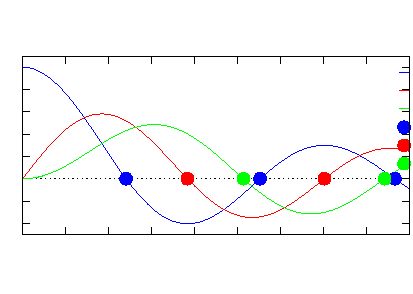
\includegraphics{Bessel-eps-converted-to.pdf}
	\caption{Illustration of the exponential function.}
\end{figure}



\end{document}